\section{Methods}

\begin{figure}[h]
    \centering
    \includegraphics[width=\linewidth]{figures/mini_pipeline.pdf}
    \caption{
        \textbf{The MINI pipeline.} \\
        \small The MINI pipeline contains 4 fairly self-explanatory steps: 1) Spatiotemporal binning and processing of neural data; 2) Training a MINI model; 3) Evaluating, and optionally re-training, the model; 4) Evaluating the model latents for interpretable features. Depending on a user's preference, steps 1-3 (including model re-training), can be either semi- or fully-automated.
    }
    \label{fig:mini_pipeline}
\end{figure}

\subsection{Neural Data Pipeline}

\subsubsection{Data Preprocessing}

Our preprocessing pipeline standardizes neural data across different recording modalities and experimental paradigms:

\begin{enumerate}
\item \textbf{Spike detection and sorting}: For raw extracellular recordings, we apply spike detection and sorting algorithms to extract single-unit activity. We use Kilosort for spike sorting followed by manual curation to ensure high-quality unit isolation.

\item \textbf{Quality control}: We filter units based on signal-to-noise ratio, isolation quality, and firing rate criteria. Units with firing rates below 0.1 Hz or above 100 Hz are excluded, as are units with poor isolation quality metrics.

\item \textbf{Binning}: Spike trains are binned at multiple temporal resolutions (1ms, 10ms, 100ms) to capture different aspects of neural dynamics. The choice of bin size depends on the temporal scale of interest and the firing characteristics of the recorded neurons.

\item \textbf{Normalization}: Neural activity is z-scored across time to account for differences in baseline firing rates across neurons. This ensures that all neurons contribute equally to the learned representations regardless of their absolute firing rates.

\item \textbf{Artifact removal}: We identify and remove periods with electrical artifacts or recording instabilities using automated detection algorithms combined with visual inspection.
\end{enumerate}

\subsubsection{Training Procedure}

Model training follows a multi-stage approach designed to optimize both reconstruction quality and feature interpretability:

\begin{enumerate}
\item \textbf{Hyperparameter optimization}: We perform systematic sweeps over key hyperparameters including sparsity weights ($\lambda$), latent dimensions ($d_{\text{sae}}$), and top-k sparsity constraints. Grid search is performed using validation data to identify optimal parameter combinations.

\item \textbf{Multi-scale training}: Models are trained jointly across all temporal scales with adaptive learning rates for each scale. This ensures that features at different temporal resolutions are learned simultaneously and can interact during the training process.

\item \textbf{Regularization}: We apply dropout (0.1-0.3), weight decay (1e-4), and early stopping to prevent overfitting. Learning rate scheduling is used to fine-tune convergence.

\item \textbf{Validation}: Training is monitored using held-out validation data (20\% of total data) to ensure generalization. We track both reconstruction metrics and feature stability across training epochs.
\end{enumerate}

\subsubsection{Model Evaluation}

\textbf{Reconstruction Quality:}
We assess reconstruction quality using multiple complementary metrics:
\begin{itemize}
\item Mean squared error (MSE) between original and reconstructed activity
\item Pearson correlation between original and reconstructed neural trajectories
\item Preservation of trial-to-trial variability structure
\item Spectral analysis to ensure temporal frequency content is preserved
\end{itemize}

\textbf{Feature Interpretability:}
Interpretability is evaluated through multiple approaches:
\begin{itemize}
\item Visual inspection of learned features and their temporal dynamics
\item Correlation analysis with known behavioral and stimulus variables
\item Consistency of features across experimental sessions and animals
\item Biological plausibility assessment based on known neural circuit properties
\end{itemize}

\textbf{Downstream Task Performance:}
We validate the utility of discovered features through:
\begin{itemize}
\item Decoding of behavioral variables (movement direction, choice, reaction time)
\item Stimulus decoding (visual scenes, auditory features, tactile inputs)
\item Cross-session and cross-animal generalization performance
\item Comparison with features from standard dimensionality reduction methods
\end{itemize}

\subsubsection{Interactive Dashboard for Feature Exploration}

To facilitate interpretation of discovered features, we develop an interactive dashboard that enables researchers to:

\begin{itemize}
\item \textbf{Visualize feature dynamics}: Interactive plots showing feature activation patterns across time, trials, and experimental conditions
\item \textbf{Correlation analysis}: Tools to correlate features with behavioral and stimulus variables, including lag analysis and significance testing
\item \textbf{Cross-model comparison}: Side-by-side comparison of features across different model configurations and hyperparameter settings
\item \textbf{Export functionality}: Export features and associated metadata for integration with external analysis pipelines
\item \textbf{Statistical summaries}: Automated generation of feature statistics including activation frequency, selectivity indices, and stability measures
\end{itemize}

The dashboard integrates seamlessly with common neuroscience analysis workflows and provides both high-level overviews and detailed single-feature analysis capabilities.


\subsection{Model architecture}

\begin{figure}[h]
    \centering
    \begin{minipage}{0.63\linewidth}
    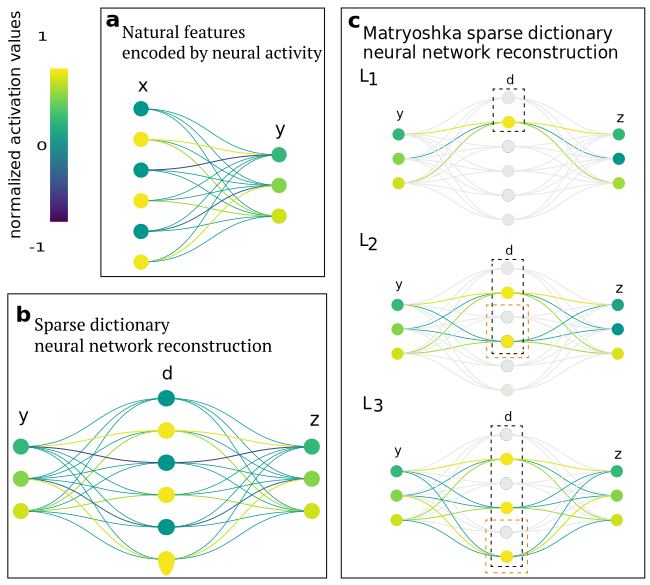
\includegraphics[width=\linewidth]{figures/sdnn_arch.pdf}
    \end{minipage}
    \begin{minipage}{0.37\linewidth}
    \caption{
        \textbf{MINI's sparse dictionary neural network architecture.} \\
        \small (\textbf{a}) Natural features $x$ get encoded by neural activity $y$. (\textbf{b}) A sparse dictionary neural network attempts to recreate neural activity $\hat{y}$ from $y$. If $\hat{y}$ tries to recreate $y$ exactly, then the model is an autoencoder, while in other situations it may be a transcoder or crosscoder. \textbf{c}) A Matryoshka spare dictionary neural network segments the latent space into multiple levels, each of which attempts to do a full reconstruction of the target neural activity. In this case, latents exclusive to the highest-level will often correspond to high-level features (e.g. a round object), while latents exclusive to the lowest-level will often correspond to low-level features (e.g. a basketball).
    }
    \label{fig:sdnn_arch}
    \end{minipage}
\end{figure}

\begin{itemize}
    \item Usefulness of SDL methods in Mech interp.
    
    \item Variant of MSAE as variant of SAE.
    \begin{itemize}
        \item Briefly mention other archs tried: batchTopK winner for sparsity enforcement.
    \end{itemize}
    
    \item In addition to MSAE levels width, briefly mention hyperparameters, expound in Appendix.
    \begin{itemize}
        \item topk per level, loss X per level, seq len for neural data, seq len for latent space used with transformer layer in decoder
    \end{itemize}
    
    \item Show latex formulas for encoder, decoder, total loss.
\end{itemize}
